\section{Introduction}
This chapter describes and outlines the requirements for the proposed software solution. Requirements will set goals for the functionality of the software, whereas the design section allows us to translate these requirements onto paper. Both sections will become useful when testing whether the system is fit-for-purpose.

\section{Requirement Methodology}
In this section, system requirements will be presented. Two sources of requirements were used: firstly using information discovered from the literature survey; and secondly from an interview from a project manager at `Company A'. These requirements are not to be used as an exhaustive list, but are to be used as a benchmark for ensuring the created product is fit-for-purpose.

\subsection{The Interview}
To gather business oriented requirements, an interview was conducted with a project manager, specialising in IT implementations for corporate facilities. several points discussed were integrated into the system as requirements. For instance:

{\fontfamily{ppl}\selectfont
6. What do you think of this solution? (The corporate loyalty app)

For this solution to be feasible and useful, it would need to be:

\begin{itemize}
\item Available for all of our permanent staff to use
\item Easy integration for further sites and users globally
\item Good usability aspects. GSK has 100,000 staff members with a variety of demographics, therefore all users should find it easy to use and better than the existing process
\item The system would need to increment on a daily basis when the staff members enter site (once a day only)
\end{itemize}
}

Informed requirements M2, S3, S4, and C4.

The transcript of the interview can be found in the appendices. 

\clearpage{}

\subsection{Requirements}
Our solution involves the creation of two Android applications, thus the requirements below will be marked whether they are for \textbf{Both} or exclusively for the \textbf{Loyalty Manager}, or \textbf{Loyalty Reader}. Effort will be made to maximise cross-system requirements. We found that there was an abundance of potential system requirements, however not all can be implemented in good time. As such, we present these requirements in MoSCoW Format~\cite{brennan2009guide} (Must Have, Should Have, Could Have, Won't Have) in order to categorise the importance of their delivery.

\subsubsection{Must Have}
\begin{description}[leftmargin=!,labelwidth=\widthof{\bfseries Medium}]
    \item[M1] \textbf{Sign-In \& Registration} \newline
        \textit{The user should be able to sign in with an existing account or register for a new one} \newline
        [Both Systems] | Functional
        
    \item[M2] \textbf{Fast Stamping} \newline
        \textit{Access to the NFC stamping functionality should be available within a single tap from a home page} \newline
        [Both Systems] | Functional
    
    \item[M3] \textbf{NFC Transmission} \newline
        \textit{The system must use NFC for data transmission and Host Card Emulation} \newline
        [Both Systems] | Functional
        
    \item[M4] \textbf{Online Syncing} \newline
        \textit{The system must be able to sync a users 'stampbook' online} \newline
        [Both Systems] | Functional
        
    \item[M5] \textbf{Sync on Interaction} \newline
        \textit{Syncing must take place as soon as there is an interaction that affects the stamp count of a scheme} \newline
        [Both Systems] | Functional
        
    \item[M6] \textbf{Syncing Time} \newline
        \textit{The response time for syncing must be within 5 seconds} \newline
        [Both Systems] | Non-functional  
        
    \item[M7] \textbf{Feedback on Interaction} \newline
        \textit{The system must provide audio/visual feedback whenever a 'stamp' has taken place} \newline
        [Both Systems] | Functional
        
\end{description}

`Must have' requirements are the minimum amount of features to be satisfied for the success of the system. As a result, these are of highest priority. Requirements defining gamification are not listed here as they are not `key' to the system.

\subsubsection{Should Have}
\begin{description}[leftmargin=!,labelwidth=\widthof{\bfseries Medium}]
    \item[S1] \textbf{Consistency} \newline
        \textit{The system should fit within the standards and design language of the Android operating system} \newline
        [Both Systems] | Non-functional
        
    \item[S2] \textbf{Secure Communications} \newline
        \textit{NFC Communications between devices should be encrypted} \newline
        [Both Systems] | Functional

    \item[S3] \textbf{Rewards Browsing} \newline
        \textit{The user should be able to easily browse their rewards available} \newline
        [Loyalty Reader] | Functional
        
    \item[S4] \textbf{Levelling System} \newline
        \textit{Users should be able to level up each of their loyalty schemes independently (20 - gold, 50, platinum)} \newline
        [Loyalty Reader] | Functional
        
    \item[S5] \textbf{Level-Restrictions} \newline
        \textit{Rewards should have a minimum-level required in order to claim} \newline
        [Loyalty Reader] | Functional

    \item[S6] \textbf{Badges} \newline
        \textit{Users should be able to collect badges upon completing certain goals} \newline
        [Loyalty Reader] | Functional
\end{description}

The `should have's' represent features which should be included if the system if time permits. Generally these requirements add a layer of usability and engagement to the system; as such, most of the gamification implementation is defined here.

\subsubsection{Could Have}
\begin{description}[leftmargin=!,labelwidth=\widthof{\bfseries Medium}]
    \item[C1] \textbf{Branding} \newline
        \textit{The system could provide deep customisation options for each scheme} \newline
        [Loyalty Manager] | Functional
        
    \item[C2] \textbf{Personalisation} \newline
        \textit{The system could allow users to customise the appearance of their profile} \newline
        [Loyalty Reader] | Functional
        
    \item[C3] \textbf{Passive Card Emulation} \newline
        \textit{The system could allow passive host card emulation} \newline
        [Loyalty Reader] | Functional
        
    \item[C4] \textbf{Restricted Schemes} \newline
        \textit{The system could allow for account-specific schemes (only authorised users have access to the scheme)} \newline
        [Both Systems] | Functional
        
    \item[C5] \textbf{Internet-Free Stamping} \newline
        \textit{Users could have the ability to gather stamps without being connected to the internet (facilitated by the Manager)} \newline
        [Loyalty Manager] | Functional
        
    \item[C6] \textbf{Multiple Device Support} \newline
        \textit{Users could be able to login and use multiple devices seamlessly} \newline
        [Loyalty Reader] | Functional
        
    \item[C7] \textbf{Transaction History} \newline
        \textit{The system could have a transaction history to allow users to see their recent activity} \newline
        [Loyalty Reader] | Functional
\end{description}

These requirements represent bells-and-whistles requirements. Features in the `could have' are desirable but not a necessity to the project's initial builds. Incorporations of these requirements into future builds of the system would greatly benefit user experience.

\subsubsection{Won't Have}
\begin{description}[leftmargin=!,labelwidth=\widthof{\bfseries Medium}]
    \item[W1] \textbf{Payment Options} \newline
        \textit{The system will not facilitate any form of payment} \newline
        [Both Systems] | Functional  
        
    \item[W2] \textbf{Loyalty Sharing} \newline
        \textit{Users will not be able to transfer stamps between friends/accounts} \newline
        [Loyalty Reader] | Functional 
\end{description}

`Won't have' requirements are simply outside the scope of the project. Their functionality is either not the purpose of the system (W1), or facilitate unwanted features into the ecosystem (W2). 






\clearpage{}
\section{Design}
\subsection{Outline}
Turning our attention to the design, here we present the system, matching the requirements, outlining how they meet the system requirements. Some interesting scenarios have been mentioned in the requirements that leave a wide scope of design challenges. A study is also undertaken that involves participatory design as an extension of the proposed design - in effect, asking potential users to tackle these challenges.


\subsection{The Three Components of the System}
As mentioned earlier, the proposed system involves two separate Android applications. However, in order to meet functional requirements M1, M4, S4, S6, C4 and C6 a database will need to be introduced in order to inter-connect user accounts, along with any relevant data (i.e. loyalty schemes, stamps and badges). Furthermore, a database is also useful from a security and continuity standpoint. For instance, backing-up stamps and schemes allows users to sync their accounts between phones, as well as preventing `abusive' users from modifying the local variables for stamp count.

\subsection{Modeling The Interaction}
The key design challenge of the system is to ensure seamless and correct communications via NFC between each of the three system modules. As outlined in the literature survey, there are several modes that NFC can adopt~\cite{MODESOFOPERATION}, each changing the device's role as part of the interaction. In this case, Host Card Emulation (HCE) and NFC Readers can be setup in different configurations to facilitate these communications. Two such configurations were considered - Loyalty Manager using HCE and Loyalty Reader using HCE (Fig. \ref{fig:dArches}). The difference between these configurations is small; however they each have distinct connotations. A discussion on their implications follows:

\begin{figure}[H]
 \centering
  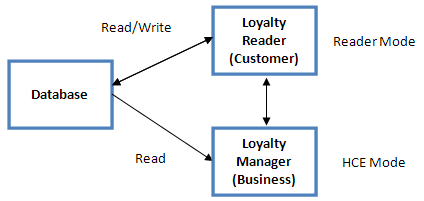
\includegraphics[width=0.48\textwidth]{img/dArch1.png}
   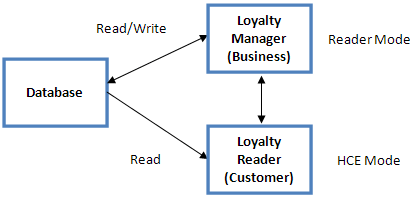
\includegraphics[width=0.48\textwidth]{img/dArch2.png}
    \caption{(i) Loyalty Manager using HCE. (ii) Loyalty Reader using HCE}
     \label{fig:dArches}
\end{figure}

\subsubsection{Loyalty Manager using HCE}
Loyalty Manager with HCE entails using the Manager application as a smartcard. In this case, the Loyalty Reader interfaces with the database to update the user's Stampbook. 

The benefits and drawbacks of this configuration are: 
\begin{description}[leftmargin=!,labelwidth=\widthof{\bfseries small}]
    \item[+] Syncing is not necessary as the Reader will always have the updated Stampbook
    \item[+] Less logic required in the Applications to direct stamps
    \item[---] Dependant on both applications having internet connection
    \item[---] The user must have the Loyalty Reader open to collect stamps
    \item[---] Data integrity issues if people maliciously modify code of the Reader
    \item[---] Differentiating between  reward \& stamp requests is difficult
\end{description}
\subsubsection{Loyalty Reader using HCE}
When the Loyalty Reader acts as the smartcard, several interactions differ. Primarily, the burden of dealing with the database is placed onto the Loyalty Manager.

The benefits and drawbacks of this configuration are: 
\begin{description}[leftmargin=!,labelwidth=\widthof{\bfseries small}]
    \item[+] The Loyalty Reader does not need to have the application open to collect a stamp, the phone functions as a passive smartcard.
    \item[+] Only the Loyalty Manager needs access to the internet. Customers will be able to collect and expend stamps whilst not connected
    \item[+] The Loyalty Manager can easily separate stamp requests from reward requests
    \item[+] Data is more secure as only the authorised Loyalty Manager has access to modify the database. Ultimately, this prevents user tampering and ensures data integrity within the system
    \item[---] Complex logic required in both applications
    \item[---] Providing specific feedback directly to the Loyalty Reader via the app is difficult
\end{description}

\subsubsection{Chosen Model}
Loyalty Reader using HCE was selected on the merit of its positives. Primarily, not requiring internet access from the customer, the ability to collect stamps without having the application open and its emphasis on security. On the other hand, it makes the implementation trickier, requiring more logic to support the two-way communications. None-the-less, we expect that this model will ultimately benefit the system by making it easier to use and understand for users.

\subsection{Design Methodology}
In order to develop the designs for the system components, we b
\subsubsection{Design Language}
One of Neilson's heuristics is `Consistency and Standards'~\cite{jakob}, in this case meaning that the solution should follow the platform conventions and design of the Android operating system. This was captured in the requirement S1. If this heuristic is met, users will feel more comfortable as the system presented to them feels familiar to use. The latest standards outlined by Google describe \emph{Material Design}~\cite{materialDesign}, a visual design language to be used with the new \emph{Android Lollipop} operating system with a goal to:
\begin{quote}
    \textit{``Develop a single underlying system that allows for a unified [user] experience across platforms and device sizes''}~\cite[Introduction]{materialDesign}
\end{quote}


\subsection{Design Process - Systems}

\subsubsection{Wire-Frame Mockups}
INSERT ORIGINAL DRAWN MOCKUPS HERE
\begin{figure}[H]
 \centering
  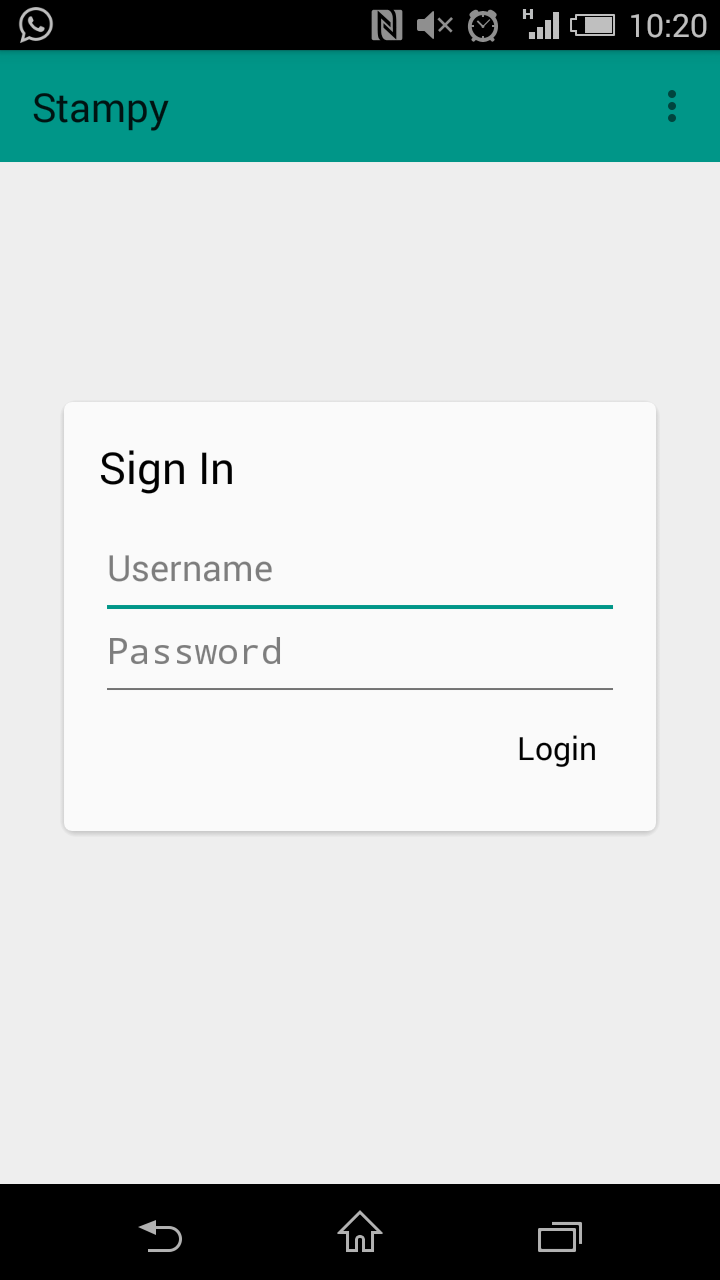
\includegraphics[width=0.24\textwidth]{img/loginMockup.png}
   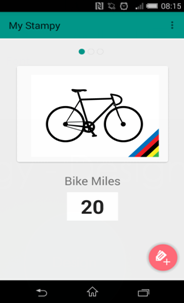
\includegraphics[width=0.24\textwidth]{img/MainMockup.png}
    \caption{Prototype}
\end{figure}

\textbf{Overview}
\subsection{Participatory Design}
\subsubsection{Need for Study/Problems With Guidelines}
\subsubsection{Aims}
\subsubsection{Outline}
\subsubsection{Results}

\subsection{Database Design}
\begin{figure}[H]
  \centering
    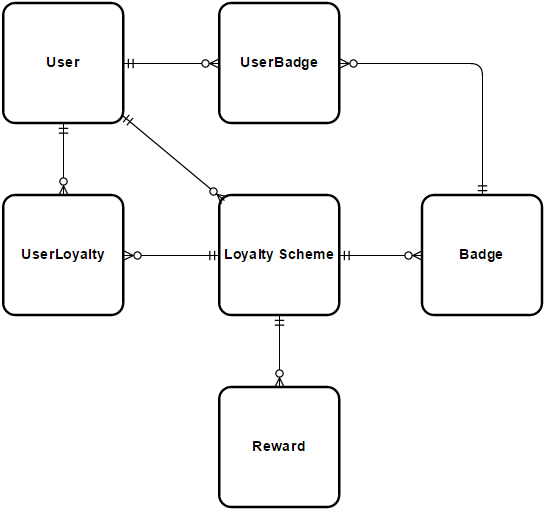
\includegraphics[width=0.5\textwidth]{img/erd.png}
      \caption{Entity Relationship Diagram}
\end{figure}
\begin{figure}[H]
  \centering
    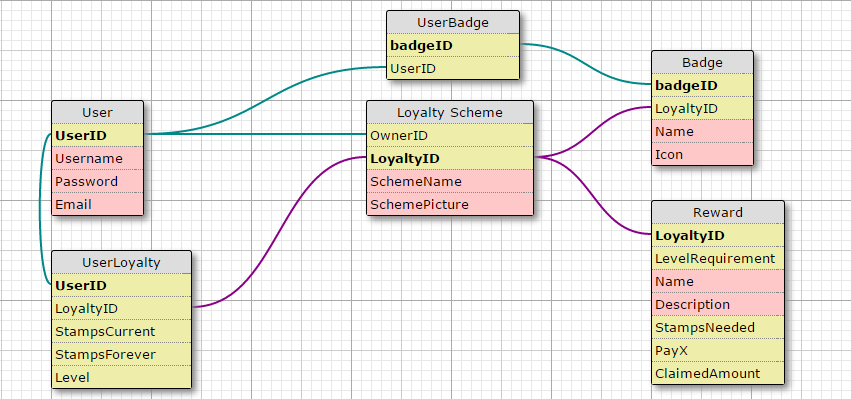
\includegraphics[width=1\textwidth]{img/architecture.png}
      \caption{Database Model}
\end{figure}